%=======================02-713 LaTeX template, following the 15-210 template==================
%
% You don't need to use LaTeX or this template, but you must turn your homework in as
% a typeset PDF somehow.
%
% How to use:
%    1. Update your information in section "A" below
%    2. Write your answers in section "B" below. Precede answers for all
%       parts of a question with the command "\question{n}{desc}" where n is
%       the question number and "desc" is a short, one-line description of
%       the problem. There is no need to restate the problem.
%    3. If a question has multiple parts, precede the answer to part x with the
%       command "\part{x}".
%    4. If a problem asks you to design an algorithm, use the commands
%       \algorithm, \correctness, \runtime to precede your discussion of the
%       description of the algorithm, its correctness, and its running time, respectively.
%    5. You can include graphics by using the command \includegraphics{FILENAME}
%
\documentclass[11pt]{article}
\usepackage{amsmath,amssymb,amsthm}
\usepackage{graphicx}
\usepackage[margin=1in]{geometry}
\usepackage{fancyhdr}
\usepackage{hyperref}
\usepackage{listings}
\usepackage{color}
\usepackage{enumerate}

\definecolor{codegreen}{rgb}{0,0.6,0}
\definecolor{codegray}{rgb}{0.5,0.5,0.5}
\definecolor{codepurple}{rgb}{0.58,0,0.82}
\definecolor{backcolour}{rgb}{0.95,0.95,0.92}

\lstdefinestyle{mystyle}{
    backgroundcolor=\color{backcolour},
    commentstyle=\color{codegreen},
    keywordstyle=\color{magenta},
    numberstyle=\tiny\color{codegray},
    stringstyle=\color{codepurple},
    basicstyle=\ttfamily\footnotesize,
    breakatwhitespace=false,
    breaklines=true,
    captionpos=b,
    keepspaces=true,
    numbers=left,
    numbersep=5pt,
    showspaces=false,
    showstringspaces=false,
    showtabs=false,
    tabsize=2
}

\lstset{style=mystyle}

\usepackage[tt=false]{libertine}

\setlength{\parindent}{0pt}
\setlength{\parskip}{5pt plus 1pt}
\setlength{\headheight}{13.6pt}
\newcommand\question[2]{\vspace{.25in}\hrule\textbf{#1. #2}\vspace{.5em}\hrule\vspace{.10in}}
\renewcommand\part[1]{\vspace{.10in}\textbf{(#1)  }}

\pagestyle{fancyplain}
\lhead{\textbf{\NAME}}
\chead{\textbf{CS229 Problem Set\#\HWNUM}}
\rhead{\today}
\fancypagestyle{plain}{%
\fancyhead{} % get rid of headers
\renewcommand{\headrulewidth}{0pt} % and the line
}

\begin{document}
%Section A==============Change the values below to match your information==================
\newcommand\NAME{Godfray Qiu}     % your name
\newcommand\STUID{}               % your student id
\newcommand\HWNUM{1}              % the homework number

%Section B==============Put your answers to the questions below here=======================


\title{\bfseries \sffamily CS 229, Autumn 2016\\Problem Set \#\HWNUM: Supervised Learning}
\author{\sffamily \NAME}

\maketitle


\question{1}{Logistic Regression}
\part{a}Consider the average empirical loss (the risk) for logistic regression:$$J(\theta) = \frac{1}{m}\sum_{i=1}^{m}\log(1+e^{-y^{(i)}\theta^Tx^{(i)}}) = -\frac{1}{m}\sum_{i=1}^{m}\log (h_{\theta}(y^{(i)}x^{(i)}))$$
where $h_{\theta}(x) = g(\theta^Tx)$ and $g(z) = 1/(1 + e^{-z})$. Find the Hessian $H$ of this function, and
show that for any vector $z$, it holds true that$$z^THz \geq 0.$$
\emph{Hint}: You might want to start by showing the fact that $\sum_{i}\sum_{j} z_ix_ix_jz_j = (x^Tz)^2 \geq 0$.

\textbf{Remark}: This is one of the standard ways of showing that the matrix $H$ is positive semi-definite, written "$H \succeq 0$". This implies that $J$ is convex, and has no local minima other than the global one \footnote{If you haven't seen this result before, please feel encouraged to ask us about it during office hours.}. If you have some other way of showing $H \succeq 0$, you're also welcome to use your method instead of the one above.

We know $g^\prime (x) = g(x)(1-g(x))$ and $g(x)+g(-x) = 1$ which may help.
$$\frac{\partial J(\theta)}{\partial \theta_k} = -\frac{1}{m}\sum_{i=1}^{m}\frac{\log(h_\theta(y^{(i)}x^{(i)}))}{\partial \theta_k} = -\frac{1}{m}\sum_{i=1}^{m}\left[1-h_\theta (y^{(i)}x^{(i)})\right]y^{(i)}x^{(i)}_{k};$$
$$\frac{\partial^2 J(\theta)}{\partial \theta_k\partial \theta_l} = \frac{\partial}{\partial \theta_l}\left(-\frac{1}{m}\sum_{i=1}^{m}\left[1-h_\theta (y^{(i)}x^{(i)})\right]y^{(i)}x^{(i)}_{k}\right) = \frac{\partial}{\partial \theta_l}\left(\frac{1}{m}\sum_{i=1}^{m}\left[h_\theta (y^{(i)}x^{(i)})\right]y^{(i)}x^{(i)}_{k}\right)$$
By rule of chain,$$H_{kl} = \frac{\partial^2 J(\theta)}{\partial \theta_k\partial \theta_l} = \frac{1}{m}\sum_{i=1}^{m}\left[y^{(i)2}h_\theta(y^{(i)}x^{(i)})\left(1-h_\theta(y^{(i)}x^{(i)})\right)x^{(i)}_{k}x^{(i)}_{l}\right]$$
After vectorization, $$H = \frac{1}{m}\sum_{i=1}^{m}\left[y^{(i)2}h_\theta(y^{(i)}x^{(i)})\left(1-h_\theta(y^{(i)}x^{(i)})\right)x^{(i)}x^{(i)T}\right]$$
Take vector $w \in \mathbb{R}^n$, $$w^THw = \frac{1}{m}\sum_{i=1}^{m}\left[y^{(i)2}h_\theta(y^{(i)}x^{(i)})\left(1-h_\theta(y^{(i)}x^{(i)})\right)w^T x^{(i)}x^{(i)T}w\right]$$
For $0<h(t)<1$ for all $t \in \mathbb{R}$, that is, $h(t)(1-h(t))>0$, and $w^T x^{(i)}x^{(i)T}w = (w^Tx^{(i)})^2 \geq 0$, $H$ is PSD.

\part{b} We have provided two data files:
\begin{itemize}
\item \href{http://cs229.stanford.edu/ps/ps1/logistic_x.txt}{logistic\_x.txt}
\item \href{http://cs229.stanford.edu/ps/ps1/logistic_y.txt}{logistic\_y.txt}
\end{itemize}
These files contain the inputs $(x^{(i)} \in \mathbb{R}^2)$ and outputs $(y(i) \in \{ -1, 1\})$, respectively for a binary classification problem, with one training example per row. Implement \footnote{Write your own version, and do not call a built-in library function.} Newton's method for optimizing $J(\theta)$, and apply it to fit a logistic regression model to the data. Initialize Newton's method with $\theta = \overrightarrow{0}$ (the vector of all zeros). What are the coefficients $\theta$ resulting from your fit? (Remember to include the intercept term.)

The Newton's method says $\theta := \theta - H^{-1}\nabla_\theta \ell(\theta)$, from (a), after 6 iterations, $\theta = [-2.6205,0.7604,1.1719]^T$.
\lstinputlisting[language=Matlab]{ps1q1b.m}

\part{c}Plot the training data (your axes should be $x_1$ and $x_2$, corresponding to the two coordinates of the inputs, and you should use a different symbol for each point plotted to indicate whether that example had label 1 or -1). Also plot on the same figure the decision boundary fit by logistic regression. (This should be a straight line showing the boundary separating the region where $h_\theta(x) > 0.5$ from where $h_\theta(x) > 0.5$.)

\begin{figure}[htbp]
  \centering
  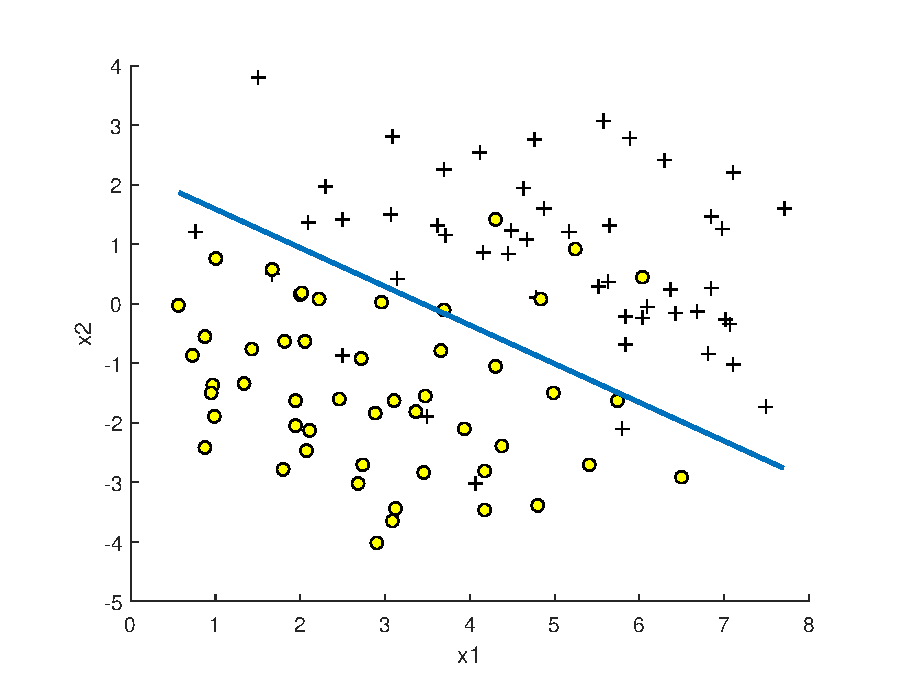
\includegraphics{ps1q1c}
  \caption{Separating hyperplane for logistic regression (question 1c).}\label{q1c}
\end{figure}

\question{2}{Poisson regression and the exponential family}
\part{a} Consider the Poisson distribution parameterized by $\lambda$:
$$p(y; \lambda) = \frac{e^{-\lambda}\lambda^y}{y!}.$$
Show that the Poisson distribution is in the exponential family, and clearly state what are $b(y)$, $\eta$, $T(y)$, and $a(\eta)$.

Usually, $p(y; \eta) = b(y)\exp{(\eta^TT(y)-a(\eta))}$, and rewrite $p$,
$$p(y; \lambda) = \frac{e^{-\lambda}\lambda^y}{y!} = \frac{\exp{(-\lambda+y\log\lambda)}}{y!}$$
So, $b(y) = 1/(y!)$, $T(y)=y$, $\eta = \log \lambda$, and $a(\eta) = \lambda = e^\eta$.

\part{b}Consider Consider performing regression using a GLM model with a Poisson response variable. What is the canonical response function for the family? (You may use the fact that a Poisson random variable with parameter $\lambda$ has mean $\lambda$.)

Canonical response function $g(\eta) = E[T(y); \eta] = E[y; \eta] = \lambda = e^\eta$.

\part{c} For a training set $\{(x^{(i)}, y^{(i)}); i = 1,\dots, m\}$, let the log-likelihood of an example be $\log p(y^{(i)}|x^{(i)}; \theta)$. By taking the derivative of the log-likelihood with respect to $\theta_j$, derive the stochastic gradient \emph{\textbf{ascent}} rule for learning using a GLM model with Poisson responses $y$ and the canonical response function.

Commonly, in stochastic gradient \emph{\textbf{ascent}}, $\theta_j := \theta_j + \alpha \frac{\partial}{\partial \theta_j}\log p(y^{(i)}|x^{(i)}; \theta)$.

In a GLM model, $h_\theta(x) = E[y | x] = \lambda = e^\eta = e^{\theta^Tx}$, and the gradient of $\theta_j$ is $(y - h_\theta(x))x_j$.

To derive, we have $\eta = \theta^Tx$, and $\frac{\partial \eta}{\partial \theta_j} = x_j$
$$\frac{\partial}{\partial \theta_j}\log p = \frac{\partial}{\partial \theta_j}\left(\eta^TT(y) - a(\eta) + \log b(y)\right) = \frac{\partial}{\partial \theta_j}\left(y\eta - a(\eta)\right) = (y - a^\prime(\eta))\frac{\partial \eta}{\partial \theta_j},$$
Common conclusion: $$\frac{\partial}{\partial \theta_j}\log p = (y - a^\prime(\eta))x_j.$$
So, $$\frac{\partial}{\partial \theta_j}\log p = (y - e^{\theta^Tx})x_j,$$
And finally, $\theta_j := \theta_j + \alpha (y - e^{\theta^Tx})x_j$ is the stochastic gradient \emph{\textbf{ascent}} rule for learning.

\part{d}Consider using GLM with a response variable from any member of the exponential family in which $T(y) = y$, and the canonical response function $h(x)$ for the family. Show that stochastic gradient ascent on the log-likelihood log $p(\overrightarrow{y}|X; \theta)$ results in the update rule $\theta_i := \theta_i - \alpha(h(x)- y)x_i$.

That is to say, the gradient of $\theta_i$ is always $(y - h_\theta(x))x_i$. In the exponential family of $T(y) = y$,
$$\frac{\partial}{\partial \theta_i}\log p = \frac{\partial}{\partial \theta_i}\left(\eta^TT(y) - a(\eta) + \log b(y)\right) = \frac{\partial}{\partial \theta_i}\left(y\eta - a(\eta)\right) = (y-\frac{\partial}{\partial \eta}a(\eta))\frac{\partial \eta}{\partial \theta_i} = (y-\frac{\partial}{\partial \eta}a(\eta))x_i,$$
We have to prove that $\frac{\partial}{\partial \eta}a(\eta)$ equals to $h_\theta(x)=g(\eta) = E[y|x;\theta]$.

Next, take from the \textsc{solution manual}:
\begin{align*}
\int_{y}p(y|x; \theta) dy &= 1\\
\int_{y}b(y)\exp(\eta^Ty-a(\eta))dy &= 1\\
\int_{y}b(y)\exp(\eta^Ty)dy &= \exp(a(\eta))
\end{align*}
Differentiating both sides with respect to $\eta$:
$$\int_{y}b(y)y\exp(\eta^Ty)dy = \exp(a(\eta))\frac{\partial a(\eta)}{\partial \eta}$$
$$\frac{\partial a(\eta)}{\partial \eta} = \int_{y}b(y)y\exp(\eta^Ty-a(\eta)) = \int_{y}yp(y|x; \theta)dy = E[y|x;\theta]$$

\question{3}{Gaussian discriminant analysis}
Suppose we are given a data set $\{(x^{(i)}, y^{(i)}); i = 1,\dots, m\}$ consisting of $m$ independent examples, where $x^{(i)} \in \mathbb{R}^n$ are $n$-dimensional vectors, and $y^{(i)} \in \{-1, 1\}$. We will model the joint distribution of $(x; y)$ according to:
\begin{align*}
  p(y) & =\left\{
               \begin{array}{ll}
                 \phi, & \hbox{if $y=1$;} \\
                 1-\phi, & \hbox{if $y=-1$.}
               \end{array}
             \right.   \\
  p(x|y=-1) & = \frac{1}{(2\pi)^{n/2}|\Sigma|^{1/2}}\exp\left(-\frac{1}{2}\left(x-\mu_{-1}\right)^T\Sigma^{-1}\left(x-\mu_{-1}\right)\right)\\
p(x|y=1) & = \frac{1}{(2\pi)^{n/2}|\Sigma|^{1/2}}\exp\left(-\frac{1}{2}\left(x-\mu_{1}\right)^T\Sigma^{-1}\left(x-\mu_{1}\right)\right)
\end{align*}
Here, the parameters of our model are $\phi$, $\Sigma$, $\mu_{-1}$ and $\mu_1$. (Note that while there're two different mean vectors $\mu_{-1}$ and $\mu_1$, there's only one covariance matrix $\Sigma$.)

\part{a} Suppose we have already fit $\phi$, $\Sigma$, $\mu_{-1}$ and $\mu_1$, and now want to make a prediction at some new query point $x$. Show that the posterior distribution of the label at $x$ takes the form of a logistic function, and can be written$$p(y | x; \phi, \Sigma, \mu_{-1}, \mu_1) = \frac{1}{1+\exp(-y(\theta^Tx+\theta_0))},$$
where $\theta \in \mathbb{R}^n$ and the bias term $\theta_0 \in \mathbb{R}$ are some appropriate functions of $\phi$, $\Sigma$, $\mu_{-1}$ and $\mu_1$. (Note: the term $\theta_0$ corresponds to introducing an extra coordinate $x^{(i)}_0 = 1$, as we did in class.)

By Bayes rule, we have $$p(y|x; \theta) = \frac{p(x|y)p(y)}{p(x)}$$
By law of total probability, we have $$p(x) = p(x|y=1)p(y=1)+p(x|y=-1)p(y=-1)$$
Considering
\begin{align*}
  p(y=1|x; \theta) &= \frac{p(x|y=1)p(y=1)}{p(x|y=1)p(y=1)+p(x|y=-1)p(y=-1)} \\
 ~& =\frac{\phi\exp\left(-\frac{1}{2}\left(x-\mu_{1}\right)^T\Sigma^{-1}\left(x-\mu_{1}\right)\right)}{\phi\exp\left(-\frac{1}{2}\left(x-\mu_{1}\right)^T\Sigma^{-1}\left(x-\mu_{1}\right)\right)+(1-\phi)\exp\left(-\frac{1}{2}\left(x-\mu_{-1}\right)^T\Sigma^{-1}\left(x-\mu_{-1}\right)\right)}
\end{align*}
We make the numerator 1, $$ p(y=1|x; \theta) = \frac{1}{1+\exp\left(\log\frac{1-\phi}{\phi}+\frac{1}{2}\left[(x-\mu_{1})^T\Sigma^{-1}(x-\mu_{1})-(x-\mu_{-1})^T\Sigma^{-1}(x-\mu_{-1})\right]\right)}$$
and $\Sigma$ is symmetric, $$\frac{1}{2}\left[(x-\mu_{1})^T\Sigma^{-1}(x-\mu_{1})-(x-\mu_{-1})^T\Sigma^{-1}(x-\mu_{-1})\right] = \frac{1}{2}\left(\mu_1^T\Sigma^{-1}\mu_1-\mu_{-1}^T\Sigma^{-1}\mu_{-1}\right)+(\mu_{-1}^T-\mu_{1}^T)\Sigma^{-1}x$$
$$p(y=1|x; \theta) = \frac{1}{1+\exp\left(\log\frac{1-\phi}{\phi}+\frac{1}{2}\left(\mu_1^T\Sigma^{-1}\mu_1-\mu_{-1}^T\Sigma^{-1}\mu_{-1}\right)+(\mu_{-1}^T-\mu_{1}^T)\Sigma^{-1}x \right)}$$
Considering factor of $-y = -1$, we get $\theta_0 = \log\frac{\phi}{1-\phi}-\frac{1}{2}\left(\mu_1^T\Sigma^{-1}\mu_1-\mu_{-1}^T\Sigma^{-1}\mu_{-1}\right)$ \\
and $\theta^T = -(\mu_{-1}-\mu_{1})^T\Sigma^{-1}$, that is $\theta = \Sigma^{-1}(\mu_{1}-\mu_{-1})$.

\part{b}For this part of the problem only, you may assume $n$ (the dimension of $x$) is 1, so that $\Sigma = [\sigma^2]$ is just a real number, and likewise the determinant of $\Sigma$ is given by $|\Sigma|=\sigma^2$. Given the data set, we claim that the maximum likelihood estimates of the parameters are given by
\begin{align*}
  \phi & = \frac{1}{m}\sum_{i=1}^{m}1\{y^{(i)} = 1\} \\
  \mu_{-1} & =\frac{\sum_{i=1}^{m}1\{y^{(i)} = -1\}x^{(i)}}{\sum_{i=1}^{m}1\{y^{(i)} = -1\}} \\
  \mu_{1} & =\frac{\sum_{i=1}^{m}1\{y^{(i)} = 1\}x^{(i)}}{\sum_{i=1}^{m}1\{y^{(i)} = 1\}} \\
  \Sigma & =\frac{1}{m}\sum_{i=1}^{m}(x^{(i)}-\mu_{y^{(i)}})(x^{(i)}-\mu_{y^{(i)}})^T
\end{align*}
The log-likelihood of the data is
\begin{align*}
  \ell(\phi, \mu_{-1}, \mu_{1}, \Sigma) & = \log \prod_{i=1}^{m}p(x^{(i)}, y^{(i)}; \phi, \mu_{-1}, \mu_{1}, \Sigma) \\
  ~ & =\log \prod_{i=1}^{m}p(x^{(i)}|y^{(i)}; \mu_{-1}, \mu_{1}, \Sigma)p(y^{(i)}; \phi)
\end{align*}
By maximizing $\ell$ with respect to the four parameters, prove that the maximum likelihood estimates of $\phi$, $\Sigma$, $\mu_{-1}$ and $\mu_1$, are indeed as given in the formulas above. (You may assume that there is at least one positive and one negative example, so that the denominators in the definitions of $\mu_{-1}$ and $\mu_1$ above are non-zero.)

\part{c}Without assuming that $n = 1$, show that the maximum likelihood estimates of $\phi$, $\Sigma$, $\mu_{-1}$ and $\mu_1$ are as given in the formulas in part (b). [Note: If you're fairly sure that you have the answer to this part right, you don't have to do part (b), since that's just a special case.]

Taken from \textsc{\textbf{solution manual}}:

$\ell(\phi, \mu_{-1}, \mu_{1}, \Sigma) \simeq$
$$ \sum_{i = 1}^{m}\left[\frac{1}{2}\log\frac{1}{|\Sigma|}-\frac{1}{2}(x^{(i)}-\mu_{y^{(i)}})^T\Sigma^{-1}(x^{(i)}-\mu_{y^{(i)}})\right]+\sum_{i = 1}^{m}\left[y^{(i)}\log\phi+(1-y^{(i)})\log(1-\phi)\right]$$
Maximizing the likelihood by setting the derivative (gradient) with respect to each of the parameters to 0.
$$\frac{\partial \ell}{\partial \phi} = \sum_{i=1}^{m}\left[\frac{y^{(i)}}{\phi}+\frac{1-y^{(i)}}{\phi-1}\right] = \frac{\sum_{i=1}^{m}1\{y^{(i)}=1\}}{\phi}+\frac{m - \sum_{i=1}^{m}1\{y^{(i)}=1\}}{\phi-1}=0,$$
We get the maximum likelihood estimates of the parameter $\phi$. And for $\mu$, by Matrix Book,
\begin{align*}
  \nabla_{\mu_1}\ell &  = -\frac{1}{2}\sum_{y^{(i)} =1} \nabla_{\mu_1}(x^{(i)}-\mu_{1})^T\Sigma^{-1}(x^{(i)}-\mu_{1})  \\
  ~ & = -\frac{1}{2}\sum_{y^{(i)} =1} \nabla_{\mu_1} \left(x^{(i)T}\Sigma^{-1}x^{(i)} - \mu_{1}^T\Sigma^{-1}x^{(i)} - x^{(i)T}\Sigma^{-1}\mu_{1}+\mu_{1}^T\Sigma^{-1}\mu_{1}\right) \\
  ~ & = -\frac{1}{2}\sum_{y^{(i)} =1}\left[2\Sigma^{-1}\mu_{1}-2\Sigma^{-1}x^{(i)}\right] = 0;
\end{align*}
Then, we will get the results of $\mu_{1}$ and $\mu_{-1}$ consistent with part(b).

The last step with respect to $\Sigma^{-1}$, denoted as $S = \Sigma^{-1}$ and $|S| = 1/|\Sigma|$,
\begin{align*}
  \nabla_{S}\ell &  = \sum_{i=1}^{m}\nabla_S\left[\frac{1}{2}\log|S|-\frac{1}{2}\underbrace{(x^{(i)}-\mu_{y^{(i)}})^T}_{b_i^T}S\underbrace{(x^{(i)}-\mu_{y^{(i)}})}_{b_i}\right]\\
~ & = \sum_{i=1}^{m}\left[\frac{1}{2|S|}\nabla_S|S|-\frac{1}{2}\nabla_Sb_i^TSb_i\right]
\end{align*}
while
$$\nabla_S|S| = |S|(S^{-1})^T$$
$$\nabla_Sb_i^TSb_i = \nabla_S tr(b_i^TSb_i)=\nabla_S tr(Sb_ib_i^T) = b_ib_i^T$$
set
$$\nabla_S\ell = \frac{1}{2}\sum_{i=1}^{m}\left[S^{-1}-b_ib_i^T\right] = 0$$
and we have $$S^{-1}=\Sigma = \frac{1}{m}\sum_{i=1}^{m}(x^{(i)}-\mu_{y^{(i)}})(x^{(i)}-\mu_{y^{(i)}})^T.$$

\question{4}{Linear invariance of optimization algorithms}
Consider using an iterative optimization algorithm (such as Newton's method, or gradient descent) to minimize some continuously differentiable function $f(x)$. Suppose we initialize the algorithm at $x^{(0)} = \overrightarrow{0}$. When the algorithm is run, it will produce a value of $x \in \mathbb{R}^n$ for each iteration: $x^{(1)}, x^{(2)}, \cdots$.
Now, let some non-singular square matrix $A \in \mathbb{R}^{n\times n}$ be given, and define a new function $g(z) = f(Az)$. Consider using the same iterative optimization algorithm to optimize $g$ (with
initialization $z^{(0)} = \overrightarrow{0}$). If the values $z^{(1)}, z^{(2)}, \cdots$ produced by this method necessarily satisfy $z^{(i)} = A^{-1}x^{(i)}$ for all $i$, we say this optimization algorithm is \textbf{invariant to linear reparameterizations}.

\part{a} Show that Newton's method (applied to find the minimum of a function) is invariant to linear reparameterizations. Note that since $z^{(0)} = \overrightarrow{0} = A^{-1}x^{(0)}$, it is sufficient to show that if Newton's method applied to $f(x)$ updates $x^{(i)}$ to $x^{(i+1)}$, then Newton's method applied to $g(z)$ will update $z^{(i)} = A^{-1}x^{(i)}$ to $z^{(i+1)} = A^{-1}x^{(i+1)}$. \footnote{Note that for this problem, you must explicitly prove any matrix calculus identities that you wish to use that are not given in the lecture notes.}

Taken from \textsc{\textbf{solution manual}}.

First, we do $\nabla_z g(z)$,
\begin{align*}
  \frac{\partial g(z)}{\partial z_i} & =  A_{*i}^T\nabla_xf(Az)\\
  \nabla_z g(z) & = A^T\nabla_x f(Az)
\end{align*}
where $A_{*i}^T$ means the i-th column of matrix $A$ and $\nabla_x f(Az)$ is the vector of $\nabla_x f(x)$ evaluated at $Az$.

Then we do $\nabla_z^2 g(z)$,
$$  H_{ij} = \frac{\partial^2 g(z)}{\partial z_i\partial z_j}  =  A_{*i}^TH_f(Az)A_{*j}$$
$$ \nabla_z^2 g(z) = A^TH_f(Az)A = H_g(z)$$
And we have
\begin{align*}
  z^{(i+1)} & = z^{(i)}-(H_g(z^{(i)}))^{-1}\nabla_z g(z^{(i)}) \\
  ~ & = z^{(i)}-A^{-1}(H_f(Az^{(i)}))^{-1}(A^T)^{-1}A^T\nabla_xf(Az^{(i)})\\
  ~ & = z^{(i)}-A^{-1}(H_f(Az^{(i)}))^{-1}\nabla_xf(Az^{(i)})
\end{align*}
So considering $Az^{(i)} = x^{(i)}$,
\begin{align*}
Az^{(i+1)} & = Az^{(i)}-AA^{-1}(H_f(Az^{(i)}))^{-1}\nabla_xf(Az^{(i)})\\
~ & = x^{(i)}-(H_f(x^{(i)}))^{-1}\nabla_xf(x^{(i)})\\
~ & = x^{(i+1)}.
\end{align*}
\part{b}Is gradient descent invariant to linear reparameterizations? Justify your answer.

No. We take
\begin{align*}
z^{(i+1)}  & = z^{(i)}-\alpha \nabla_z g(z^{(i)})\\
~ & = z^{(i)}-\alpha A^T\nabla_x f(Az^{(i)})\\
Az^{(i+1)} & = Az^{(i)}-\alpha AA^T\nabla_x f(Az^{(i)})\\
~ & = x^{(i)}-\alpha AA^T\nabla_x f(x^{(i)})
\end{align*}
while $$x^{(i+1)} = x^{(i)}-\alpha \nabla_x f(x^{(i)})$$
If and only if $AA^T=I$ it holds. That is to say $A$ is orthogonal.

\newpage
\question{5}{Regression for denoising quasar spectra\footnote{Ciollaro, Mattia, et al. "Functional regression for quasar spectra." arXiv:1404.3168 (2014).}}
\textbf{Introduction.} In this problem, we will apply a supervised learning technique to estimate the light spectrum of quasars. Quasars are luminous distant galactic nuclei that are so bright, their light overwhelms that of stars in their galaxies. Understanding properties of the spectrum of light emitted by a quasar is useful for a number of tasks: first, a number of quasar properties can be estimated from the spectra, and second, properties of the regions of the universe through which the light passes can also be evaluated (for example, we can estimate the density of neutral and ionized particles in the universe, which helps cosmologists understand the evolution and fundamental laws governing its structure). The light spectrum is a curve that relates the light's intensity (formally, lumens per square meter), or \emph{luminous flux}, to its wavelength. Figure \ref{pic} shows an example of a quasar light spectrum, where the wavelengths are measured in Angstroms ({\AA}), where $1{\text{\AA}}= 10^{-10}$ meters.
\begin{figure}[htbp]
  \centering
  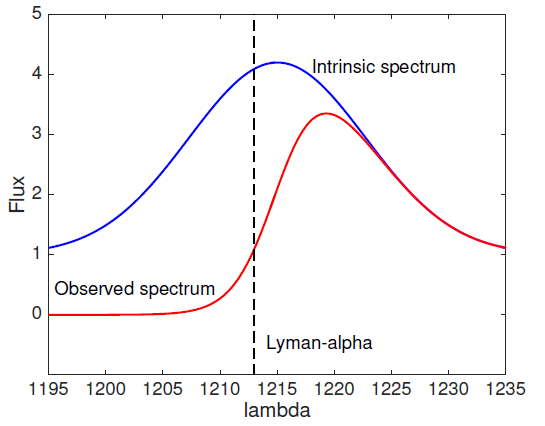
\includegraphics{ps1pic}
  \caption{Light spectrum of a quasar. The blue line shows the intrinsic (i.e. original) flux spectrum emitted by the quasar. The red line denotes the observed spectrum here on Earth. To the left of the Lyman-$\alpha$ line, the observed
flux is damped and the intrinsic (unabsorbed) flux continuum is not clearly recognizable (red line). To the right of the Lyman-$\alpha$ line, the observed flux approximates the intrinsic spectrum.}\label{pic}
\end{figure}

The Lyman-$\alpha$ wavelength is a wavelength beyond which intervening particles at most negligibly interfere with light emitted from the quasar. (Interference generally occurs when a photon is absorbed by a neutral hydrogen atom, which only occurs for certain wavelengths of light.) For wavelengths greater than this Lyman-$\alpha$ wavelength, the observed light spectrum fobs can be modeled as a smooth spectrum $f$ plus noise:
$$f_{\text{obs}}(\lambda) = f(\lambda)+ \text{noise}(\lambda)$$
For wavelengths below the Lyman-$\alpha$ wavelength, a region of the spectrum known as the Lyman-$\alpha$ forest, intervening matter causes attenuation of the observed signal. As light emitted by the quasar travels through regions of the universe richer in neutral hydrogen, some of it is absorbed,which we model as
$$f_\text{obs}(\lambda) = \text{absorption}(\lambda) \cdot f(\lambda) + \text{noise}(\lambda)$$
Astrophysicists and cosmologists wish to understand the absorption function, which gives information about the Lyman-$\alpha$ forest, and hence the distribution of neutral hydrogen in otherwise unreachable regions of the universe. This gives clues toward the formation and evolution of the universe. Thus, it is our goal to estimate the spectrum f of an observed quasar.

\textbf{Getting the data.} We will be using data generated from the Hubble Space Telescope Faint Object Spectrograph (HST-FOS), Spectra of Active Galactic Nuclei and Quasars.\footnote{https://hea-www.harvard.edu/FOSAGN/} We have provided two comma-separated data files located at:
\begin{itemize}
\item Training set: \href{http://cs229.stanford.edu/ps/ps1/quasar_train.csv}{\texttt{http://cs229.stanford.edu/ps/ps1/quasar\_train.csv}}
\item Test set:  \href{http://cs229.stanford.edu/ps/ps1/quasar_test.csv}{\texttt{http://cs229.stanford.edu/ps/ps1/quasar\_test.csv}}
\end{itemize}

Each file contains a single header row containing 450 numbers corresponding integral wavelengths in the interval $[1150, 1600]$ \AA. The remaining lines contain relative flux measurements for each wavelength. Specifically, \texttt{quasar\_train.csv} contains 200 examples and \texttt{quasar\_test.csv} contains 50 examples. You may use the helper file load quasar \texttt{data.m} to load the data in Matlab: \href{http://cs229.stanford.edu/ps/ps1/load_quasar_data.m}{\texttt{load\_quasar\_data.m}}

\part{a} Locally weighted linear regression

Consider a linear regression problem in which we want to "weight" different training examples differently. Specifically, suppose we want to minimize
$$J(\theta) = \frac{1}{2}\sum_{i=1}^{m}w^{(i)}\left(\theta^Tx^{(i)}-y^{(i)}\right)^2$$
In class, we worked out what happens for the case where all the weights (the $w^{(i)}$'s) are the
same. In this problem, we will generalize some of those ideas to the weighted setting.
\begin{enumerate}[i.]
  \item Show that $J(\theta)$ can also be written
$$J(\theta) = (X\theta-\overrightarrow{y})^TW(X\theta-\overrightarrow{y})$$
for an appropriate diagonal matrix $W$, and where $X$ and $\overrightarrow{y}$ are as defined in class. State clearly what $W$ is.

Take $W_{ii} = \frac{1}{2}w^{(i)}$ and $W_{ij} = 0$ for $i \neq j$.
\begin{align*}
  (X\theta-\overrightarrow{y})^TW(X\theta-\overrightarrow{y}) & =  (X\theta-\overrightarrow{y})^T\frac{1}{2}\text{diag}(w^{(1)}, \cdots, w^{(n)})(X\theta-\overrightarrow{y})\\
  ~ & = \frac{1}{2} \sum_{i=1}^{m}w^{(i)}\left(\theta^Tx^{(i)}-y^{(i)}\right)^2 = J(\theta)\\
\end{align*}
  \item If all the $w^{(i)}$'s equal 1, then we saw in class that the normal equation is
$$X^TX\theta = X^T\overrightarrow{y},$$
and that the value of $\theta$ that minimizes $J(\theta)$ is given by $(X^TX)^{-1}X^T\overrightarrow{y}$. By finding
the derivative $\nabla_\theta J(\theta)$ and setting that to zero, generalize the normal equation to this
weighted setting, and give the new value of $\theta$ that minimizes $J(\theta)$ in closed form as a function of $X$, $W$ and $\overrightarrow{y}$.
\begin{align*}
\nabla_\theta J(\theta) & = \nabla_\theta(\theta^TX^TWX\theta-y^TWX\theta-\theta^TX^TWy+y^TWy) \\
~ & = 2X^TWX\theta - 2X^TWy = 0,( W \text{ is symmetric }, W^T = W)
\end{align*}
Thus, $X^TWX\theta = X^TW^Ty$, that is $\theta = (X^TWX)^{-1}X^TWy$

  \item Suppose we have a training set $\{(x^{(i)}, y^{(i)}); i = 1, \cdots, m\}$ of $m$ independent examples, but in which the $y^{(i)}$'s were observed with differing variances. Specifically, suppose that
$$p(y^{(i)} | x^{(i)}; \theta) = \frac{1}{\sqrt{2\pi}\sigma^{(i)}}\exp\left(-\frac{(y^{(i)}-\theta^Tx^{(i)})^2}{2(\sigma^{(i)})^2}\right)$$
I.e., $y^{(i)}$ has mean $\theta^Tx^{(i)}$ and variance $(\sigma^{(i)})^2$ (where the $\sigma^{(i)}$'s are fixed, known, constants). Show that finding the maximum likelihood estimate of $\theta$ reduces to solving a weighted linear regression problem. State clearly what the $w^{(i)}$'s are in terms of the $\sigma^{(i)}$'s.

We first make $\ell(\theta) = \log p(y^{(i)} | x^{(i)}; \theta)$, maximizing $\ell(\theta)$
\begin{align*}
  \arg \max_{\theta} \prod_{i=1}^{m} p & = \arg \max_{\theta} \sum_{i=1}^{m}\ell({\theta})\\
  ~ & = \arg \max_{\theta} \sum_{i=1}^{m}\left( \log \frac{1}{\sqrt{2\pi}\sigma^{(i)}} - \frac{(y^{(i)}-\theta^Tx)^2}{2(\sigma^{(i)})^2}\right) \\
  ~ & = \arg \min_{\theta} \frac{1}{2}\sum_{i=1}^{m} \frac{1}{(\sigma^{(i)})^2}(y^{(i)}-\theta^Tx)^2\\
  ~ & = \arg \min_{\theta} \frac{1}{2}\sum_{i=1}^{m} w^{(i)}(y^{(i)}-\theta^Tx)^2
\end{align*}
and we have $w^{(i)} = \frac{1}{(\sigma^{(i)})^2}$, and that is a weighted linear regression.
\end{enumerate}

\part{b}Visualizing the data
\begin{enumerate}[i.]
  \item Use the normal equations to implement (unweighted) linear regression ($y = \theta^T x$) on the \emph{first} training example (i.e. first non-header row). On one figure, plot both the raw data and the straight line resulting from your fit. State the optimal $\theta$ resulting from the linear regression.
\begin{figure}[htb]
  \centering
  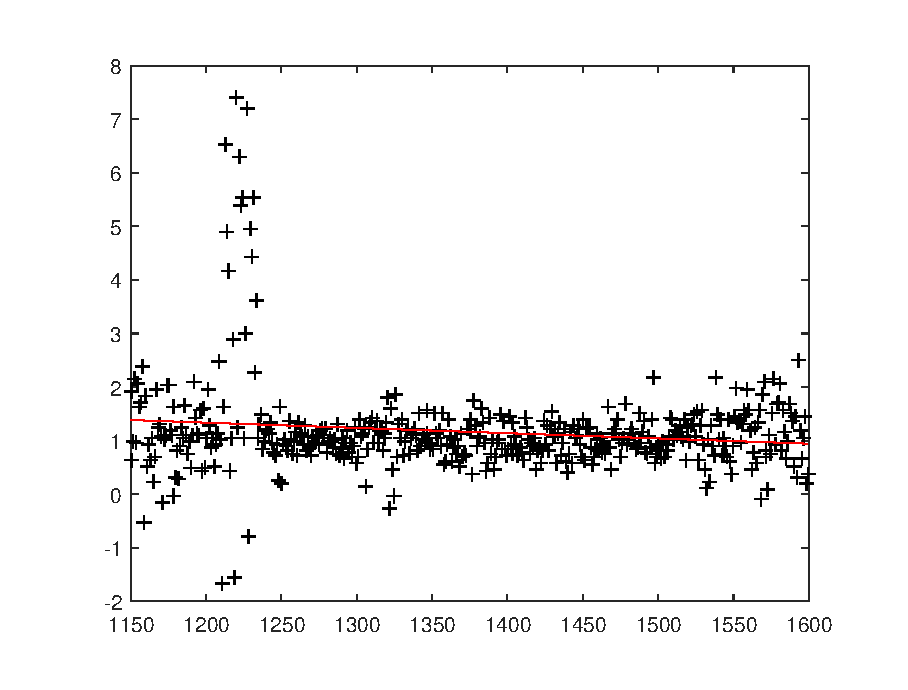
\includegraphics{ps1q5pbi}
  \caption{Regression $\theta = [2.5134 ,-0.0010]^T$.}\label{ps1q5pbi}
\end{figure}

See Figure \ref{ps1q5pbi}.

  \item Implement locally weighted linear regression on the \emph{first} training example. Use the normal equations you derived in part(a)(ii). On a different figure, plot both the raw data and the smooth curve resulting from your fit. When evaluating $h(\cdot)$ at a query point $x$, use weights $$w^{(i)} = \exp\left(-\frac{(x-x^{(i)})^2}{2\tau^2}\right)$$
      with bandwidth parameter $\tau$ = 5.

See next part of Figure \ref{ps1q5pb23}.
  \item Repeat (b)(ii) four more times with $\tau$ = 1, 10, 100 and 1000. Plot the resulting curves. You can submit one plot with all four $\tau$ values or submit four separate plots. If you submit one plot, make sure all curves are visible. Additionally, in \textbf{2-3 sentences}, comment on what happens to the locally weighted linear regression line as $\tau$ varies.
\begin{figure}[htb]
  \centering
  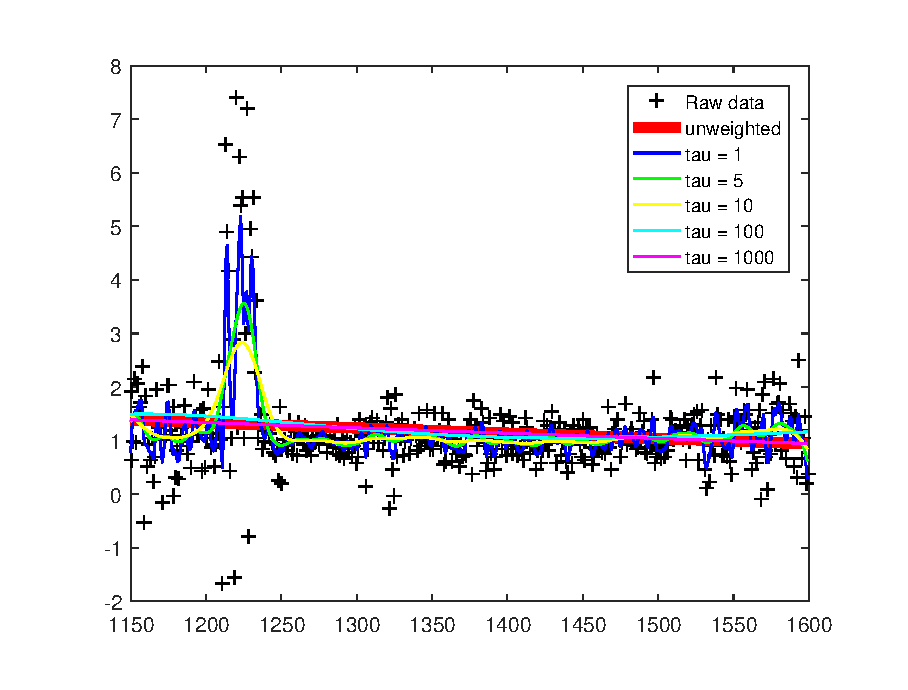
\includegraphics{ps1q5pb23}
  \caption{Varing $\tau$.}\label{ps1q5pb23}
\end{figure}

See Figure \ref{ps1q5pb23}.

Conclusion: As $\tau$ becomes large, locally weighted linear regression becomes unweighted linear regression. As $\tau$ becomes small, it begins to overfit the data.

Matlab code for this part:
\lstinputlisting[language=Matlab]{weighted_regression.m}
\lstinputlisting[language=Matlab]{ps1q5b.m}

\end{enumerate}

\part{c}Predicting quasar spectra with functional regression

We now go a step beyond what we have covered explicitly in class, and we wish to predict an entire part of a spectrum-a curve-from noisy observed data. We begin by supposing that we observe a random sample of $m$ absorption-free spectra, which is possible for quasars very close (in a sense relative to the size of the universe!) to Earth. For a given spectrum $f$, define $f_\text{right}$ to be the spectrum to the right of the Lyman-$\alpha$ line. Let $f_\text{left}$ be the spectrum within the Lyman-$\alpha$ forest region, that is, for lower wavelengths. To make the results cleaner, we define:$$f(\lambda) = \left\{
                                                     \begin{array}{ll}
                                                       f_\text{left}(\lambda), & \hbox{if $\lambda <1200$;} \\
                                                       f_\text{right}(\lambda), & \hbox{if $\lambda \geq 1300$.}
                                                     \end{array}
                                                   \right.$$
We will learn a function $r$ (for regression) that maps an observed $f_\text{right}$ to an unobserved target $f_\text{left}$. This is useful in practice because we observe $f_\text{right}$ with \emph{only} random noise: there is no systematic absorption, which we cannot observe directly, because hydrogen does not absorb photons with higher wavelengths. By predicting $f_\text{left}$ from a noisy version of $f_\text{right}$, we can estimate the unobservable spectrum of a quasar as well as the absorption function. Imaging systems collect data of the form
$$f_\text{obs}(\lambda) = \text{absorption}(\lambda) \cdot f(\lambda) + \text{noise}(\lambda)$$
for $\lambda \in \{\lambda_1, \cdots, \lambda_n\}$, a \emph{finite} number of points $\lambda$, because they must quantize the information. That is, even in the quasars-close-to-Earth training data, our observations of $f_\text{left}$ and $f_\text{right}$ consist of noisy evaluations of the true spectrum $f$ at multiple wavelengths. In our case, we have $n = 450$ and $\lambda_1 = 1150, \cdots, \lambda_n = 1599$.

We formulate the functional regression task as the goal of learning the function $r$ mapping $f_\text{left}$ to $f_\text{right}$:
$$r(f_\text{right})(\lambda) = \mathbb{E}(f_\text{left} | f_\text{right})(\lambda)$$
for $\lambda$ in the Lyman-$\alpha$ forest.
\begin{enumerate}[i.]
  \item First, we must smooth the data in the training data set to make it more useful for prediction. For each $i = 1, \cdots,m$, define $f^{(i)}(\lambda)$ to be the weighted linear regression estimate the $i^{th}$ spectrum. Use your code from part (b)(ii) above to smooth all spectra in the training set using $\tau$ = 5. Do the same for the test set. We will now operate on these smoothed spectra.
  \item Using your estimated regression functions $f^{(i)}$ for $i = 1, \cdots, m$, we now wish to estimate the unobserved spectrum $f_\text{left}$ of a quasar from its (noisy) observed spectrum $f_\text{right}$. To do so, we perform a weighted regression of the locally weighted regressions. In particular, given a new noisy spectrum observation:
$$f_\text{obs}(\lambda) = f(\lambda) + \text{noise}(\lambda)\ \text{ for } \ \lambda \in \{1300, \cdots, 1599\}. $$
We define a metric $d$ which takes as input, two spectra $f_1$ and $f_2$, and outputs a scalar:
$$d(f_1,f_2) = \sum_{i}\left(f_1(\lambda_i)-f_2(\lambda_i)\right)^2$$
The metric $d$ computes squared distance between the new datapoint and previous datapoints. If $f_1$ and $f_2$ are right spectra, then we take the preceding sum only over $\lambda \in \{1300, \cdots, 1599\}$ rather than the entire spectrum.

Based on this distance function, we may define the nonparametric \emph{functional} regression estimator, which is a locally weighted sum of \emph{functions} $f_\text{left}$ from the training data (this is like locally weighted linear regression, except that instead of predicting $y \in \mathbb{R}$ we predict a function $f_\text{left}$). Specifically, let $f_\text{right}$ denote the right side of a spectrum, which we have smoothed using locally weighted linear regression (as you were told to do in the previous part of the problem). We wish to estimate the associated \emph{left} spectrum $f_\text{left}$. Define the function $\text{ker}(t) = \max\{1-t, 0\}$ and let $\text{\texttt{neighb}}_k(f_\text{right})$ denote the $k$ indices $i \in \{1, \cdots, m\}$ that are closest to $f_\text{right}$, that is
$$d(f_\text{right}^{(i)}, f_\text{right}) < d(f_\text{right}^{(j)}, f_\text{right})\text{ for all } i \in \text{\texttt{neighb}}_k(f_\text{right}), j \notin \text{\texttt{neighb}}_k(f_\text{right})$$
and $\text{\texttt{neighb}}_k(f_\text{right})$ contains exactly $k$ indices. In addition, let
$$h := \max_{i \in \{1, \cdots, m\}} d(f_\text{right}^{(i)}, f_\text{right}).$$
Then define the estimated function $\widehat{f_\text{left}} : \mathbb{R}\rightarrow \mathbb{R}$ by
$$\widehat{f_\text{left}}(\lambda) = \frac{\sum_{i \in \text{\texttt{neighb}}_k(f_\text{right})}\text{ker}(d(f_\text{right}^{(i)}, f_\text{right})/h)f_\text{left}^{(i)}(\lambda)}{\sum_{i \in \text{\texttt{neighb}}_k(f_\text{right)}}\text{ker}(d(f_\text{right}^{(i)}, f_\text{right})/h)}$$
Recall that $f_\text{right}^{(i)}$ is the smoothed (weighted linear regression) estimate of the $i$th training spectrum.
Construct the functional regression estimate (21) for each spectrum in the entire training set using $k = 3$ nearest neighbors: for each $j = 1, \cdots, m$, construct the estimator $\widehat{f_\text{left}}$ from (21) using $f_\text{right} = f_\text{right}^{(i)}$. Then compute the error $d(f_\text{left}^{(j)}, \widehat{f_\text{left}})$ between the true spectrum $f_\text{left}^{(j)}$ and your estimated spectrum $\widehat{f_\text{left}}$ for each $j$, and return the average over the training data. What is your average training error?

Average training error is 1.0709, a little different with the \textsc{\textbf{solution manual}}...

\item Perform functional regression on the test set using the same procedure as in the previous subquestion. What is your average test error? For test examples 1 and 6, include a plot with both the entire smooth spectrum and the fitted curve $\widehat{f_\text{left}}$ curve on the same graph. You should submit two plots: one for test example 1 and one for test example 6.

Average test error is 3.0937, a little different with the \textsc{\textbf{solution manual}}...

Fitted $\widehat{f_\text{left}}$ curve:
\begin{figure}[htb]
  \centering
  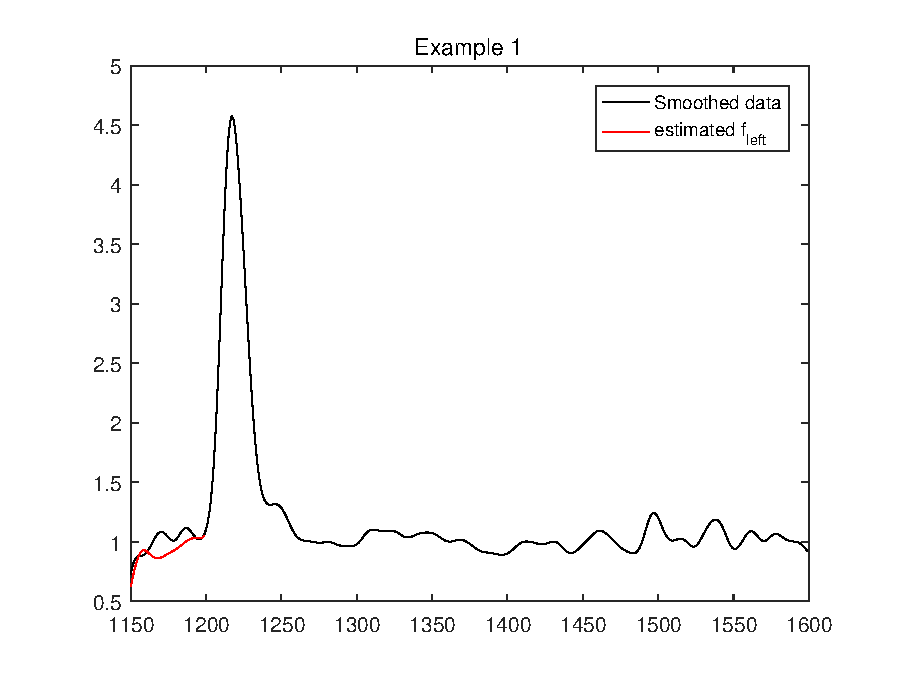
\includegraphics{ps1q5pciiiex1}
  \caption{Resulting functional regression for test set example 1.}\label{ps1q5pciiiex1}
\end{figure}
\begin{figure}[htb]
  \centering
  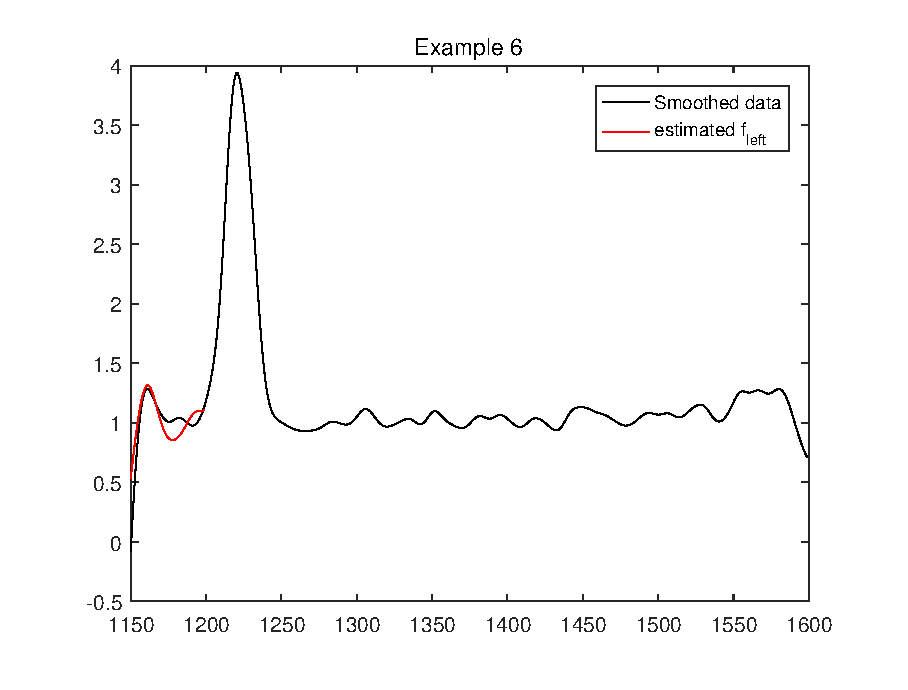
\includegraphics{ps1q5pciiiex6}
  \caption{Resulting functional regression for test set example 6.}\label{ps1q5pciiiex6}
\end{figure}

Matlab code for this part:
\lstinputlisting[language=Matlab]{ps1q5c.m}



      
      
\end{enumerate}



\end{document}
